%!TEX root = ../thesis.tex

\chapter{Implementierung} \label{sec:impl}

%%%%%%%%%%%%%%%%%%%%%%%%%%%%%%%%%%%%%%%%%%%%%%%%%%%%%%%%%%%%%
\section{Architektur \& Moduldesign} \label{sec:march}

Das Ziel der Abstraktion in einzelne Module ist es, die ``atomaren'' mathematischen Operationen zu kapseln und von der Steuerungslogik zu trennen. Die Einbindung der Hardware-Module erfolgt dadurch über wenig VHDL-Code, sodass die Steuerungsmodule übersichtlich bleiben. Die Zielarchitektur kann dabei wie folgt aussehen: \\

\begin{figure}[H]
	\centering
  	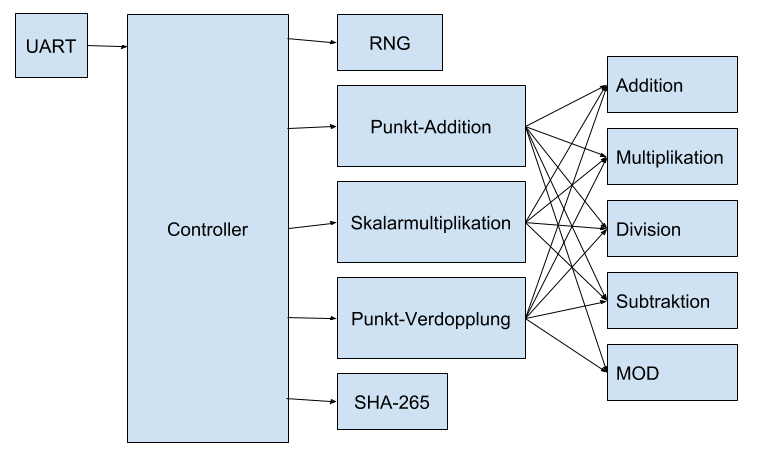
\includegraphics[width=0.9\textwidth]{bilder/opmodules}
	\caption{Zielarchitektur der FPGA-Hardware}
	\label{fig:arch}
\end{figure}

Abbildung \ref{fig:arch} zeigt einen zentralen Controller, der die einzelnen Module benutzt. Der Controller spricht dabei die mathematischen Module an, die konkret für die ECDSA-Implementierung benötigt werden. Dazu werden die atomaren Operationen (Addition, Multiplikation, Division, Subtraktion, Modulo) jeweils eingebunden, um ein höheres Abstraktionsniveau zu erhalten. Das UART-Modul repräsentiert die Kommunikation nach außen. \\

Um den ECDS-Algorithmus optimal zu implementieren, muss auf der Hardware ein ``echter'' Zufallszahlengenerator\footnote{engl. Random Number Generator, RNG} vorhanden sein, um den geheimen Schlüssel richtig zu generieren. Außerdem soll der Controller mit einer beliebig langen Nachricht umgehen und den Algorithmus zum Signieren auf einem kryptographisch sicheren Hashwert ausführen können. Da der Fokus dieser Arbeit auf Implementierung und Vergleich der ECDSA-Kernkomponenten liegt, wird aus Komplexitäts- und Platzgründen\footnote{Chipfläche auf dem zur Verfügung stehenden FPGA} auf beide vorangegangenen Features verzichtet. \\

Die Hardware-Implementierung kann eine Nachricht konstanter Länge, der einem Hash der eigentlichen Nachricht entspricht, entgegennehmen und sendet nach der Berechnung den Punkt $(r,s)$ als Antwort zurück. Bei der Verifizierung werden Nachricht und die Werte $r$ und $s$ entgegen genommen und das Ergebnis der Verifizierung (wahr oder falsch) zurück geschickt. \\

\begin{figure}[thb]
	\centering
  	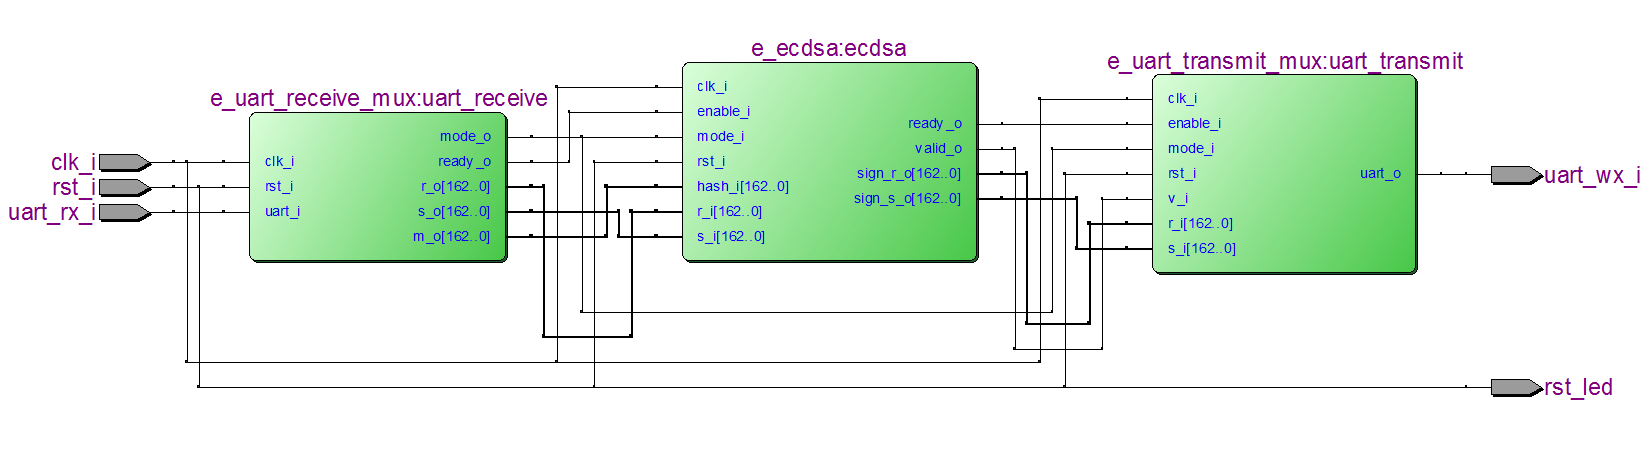
\includegraphics[width=\textwidth]{bilder/tle}
	\caption{Top-Level-Entity der VHDL-Lösung des ECDSA}
	\label{fig:tle}
\end{figure}

Die Top-Level-Entität erhält die Daten über eine serielle RS232-Schnittstelle im Modul \texttt{e\_uart\_receive\_mux} (vgl. Abb. \ref{fig:arch}). Nach vollständigem Erhalt der Daten werden diese dem zentralen Modul \texttt{e\_ecdsa} bereitgestellt und die Berechnung über ein Flag gestartet. Signalisiert das Modul die Fertigstellung der Berechnungen, wird das Modul \texttt{e\_uart\_transmit\_mux} getriggert, welches die Übertragung des Ergebnisses durchführt (vgl. Kap. \ref{sec:uart}). \\


%%%%%%%%%%%%%%%%%%%%%%%%%%%%%%%%%%%%%%%%%%%%%%%%%%%%%%%%%%%%%
\section{VHDL-Komponenten des ECDSA}

% TODO: die wichtigsten komponenten als subsection erklären
\subsection{Addierer}

\subsection{Multiplizierer}

\subsection{ECDSA Komponenten...}



%%%%%%%%%%%%%%%%%%%%%%%%%%%%%%%%%%%%%%%%%%%%%%%%%%%%%%%%%%%%%
\section{Kommunikation der UART-Verbindung} \label{sec:uartimpl}

Die UART-Komponenten übernehmen wie in Kap. \ref{sec:iuart} beschrieben neben der externen Kommunikation auch die Transformation der Daten. Dabei wird der Rx-Input\footnote{Das Rx-Signal wird erst nach Einsynchronisation mit zwei aufeinanderfolgenden Flip-Flops verarbeitet.} nach dem Empfangen über Register mit einem Parallel-Ausgang zur Verfügung gestellt. Abbildung \ref{fig:uartrx} zeigt die Verschaltung des \textbf{Receivers} mit den Schieberegistern im RTL Viewer der Entwicklungsumgebung. \\

\begin{figure}[thb]
	\centering
  	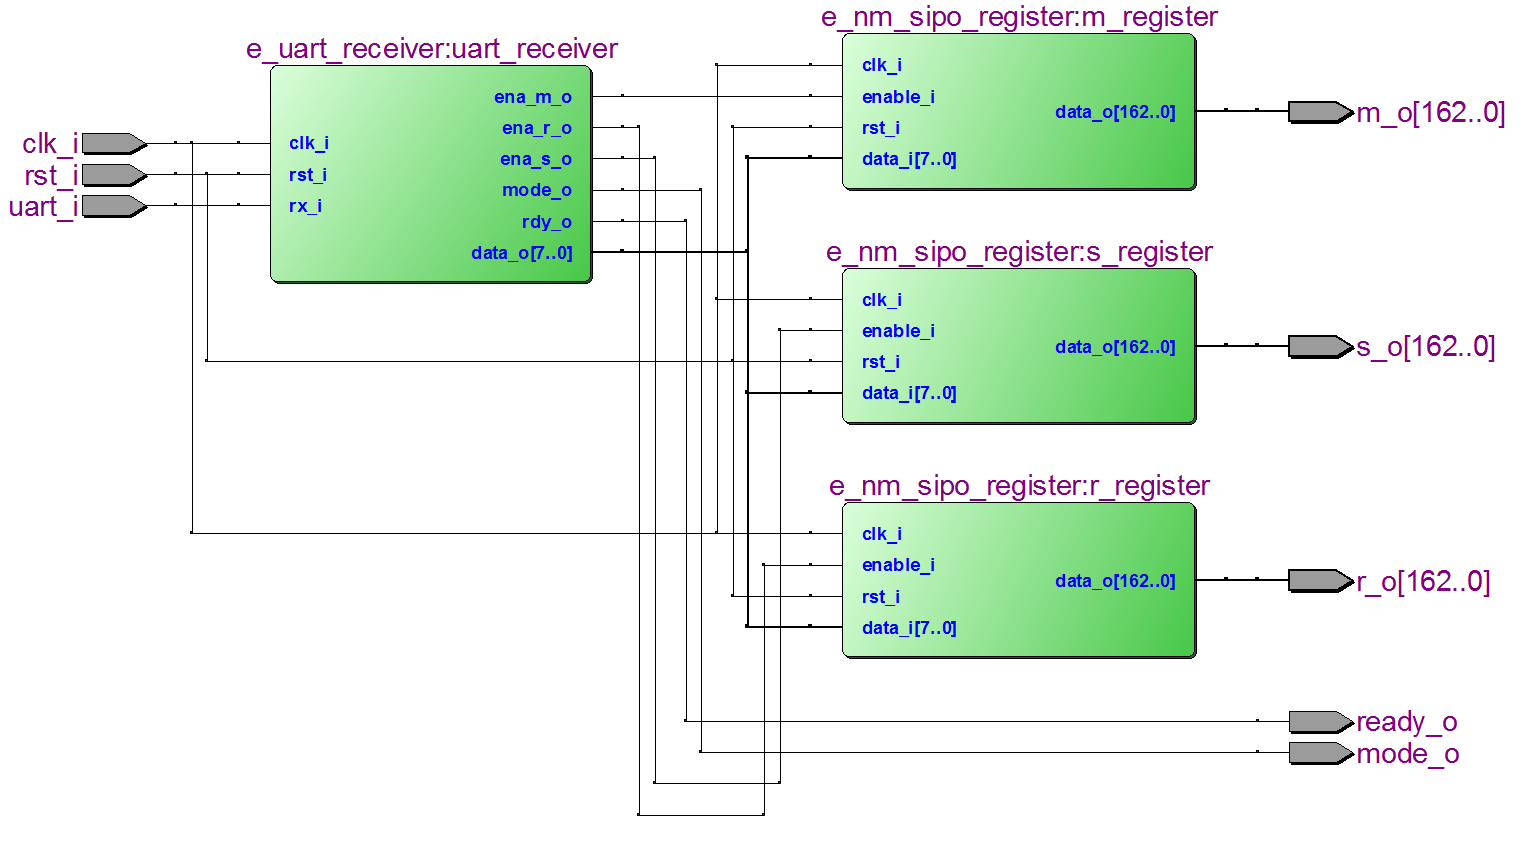
\includegraphics[width=0.9\textwidth]{bilder/uart-receiver}
	\caption{Ansicht des UART-Receivers im RTL Viewer}
	\label{fig:uartrx}
\end{figure}

Der Receiver selbst enthält einen Zustandsautomaten, der den Eingabedatenstrom in die zwei Modi \texttt{Signieren} und \texttt{Verifizieren} klassifiziert. Anhand der Zustände werden die Steuerungssignale am Modulausgang (\textit{enable}-Signale für die Punkte $r$ und $s$ auf der elliptischen Kurve sowie die Nachricht) so geschaltet, sodass jeweils die entsprechenden Eingabewörter in den dafür vorgesehenen Registern landen\footnote{phase1 = $r$, phase2 = $s$, phase3 = $message$} (vgl. Abb. \ref{fig:uart-receiver-phase}. Hierfür gibt es zwei vorangegangene Phase, in denen der Modus durch das erste empfangene Byte bestimmt wird (\textit{dmode}) und anschließend über die Dauer eines Taktzyklus umgeschaltet wird (\textit{smode}). \\

\begin{figure}[thb]
	\centering
  	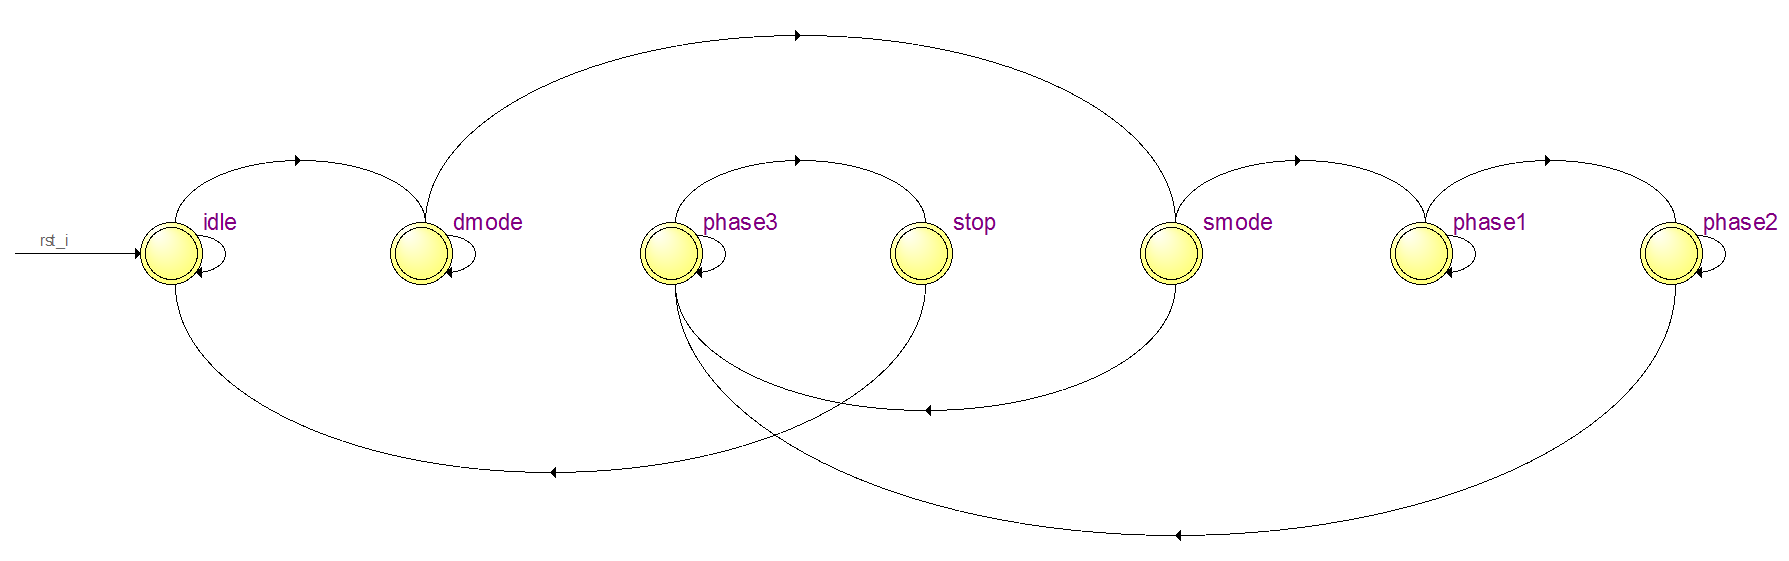
\includegraphics[width=\textwidth]{bilder/uart-receiver-phase}
	\caption{Zustandsautomat des Receivers zu Phasen-Bestimmung beim Empfang}
	\label{fig:uart-receiver-phase}
\end{figure}

Die Phasen des gezeigten Automaten bilden eine Abstraktionsebene über der eigentlichen Erkennung der sequentiellen Datenbits am Rx-Eingang. Ein weiterer Zustandsautomat (s. Anhang \ref{fig:uart-receiver-data}) agiert innerhalb eines UART-Datenpaketes (Start-Bit, 8 Bit Daten, Stop-Bit) und speichert ein einzelnes Byte zwischen zur Weiterverarbeitung. Der erste Byte für den Modus muss dabei entweder ``00000000b'' für das Signieren oder ``11111111b'' für das Verifizieren sein. Der Modus wird als binäres Signal für nachfolgende Module nach außen geführt. \\

Der \textbf{UART-Transmitter} beinhaltet zwei Schieberegister, die einen parallelen Eingang mit einem Byte-weise seriellen Ausgang besitzen (vgl. Abb. \ref{fig:uarttx}). Das \texttt{e\_uart\_transmit}-Modul steuert diese Register über einen internen Zustandsautomaten gibt die entsprechenden Steuerungssignale nach außen an die beiden Multiplexer, welche die \textit{enable}-Eingänge anspricht. \\

\begin{figure}[H]
	\centering
  	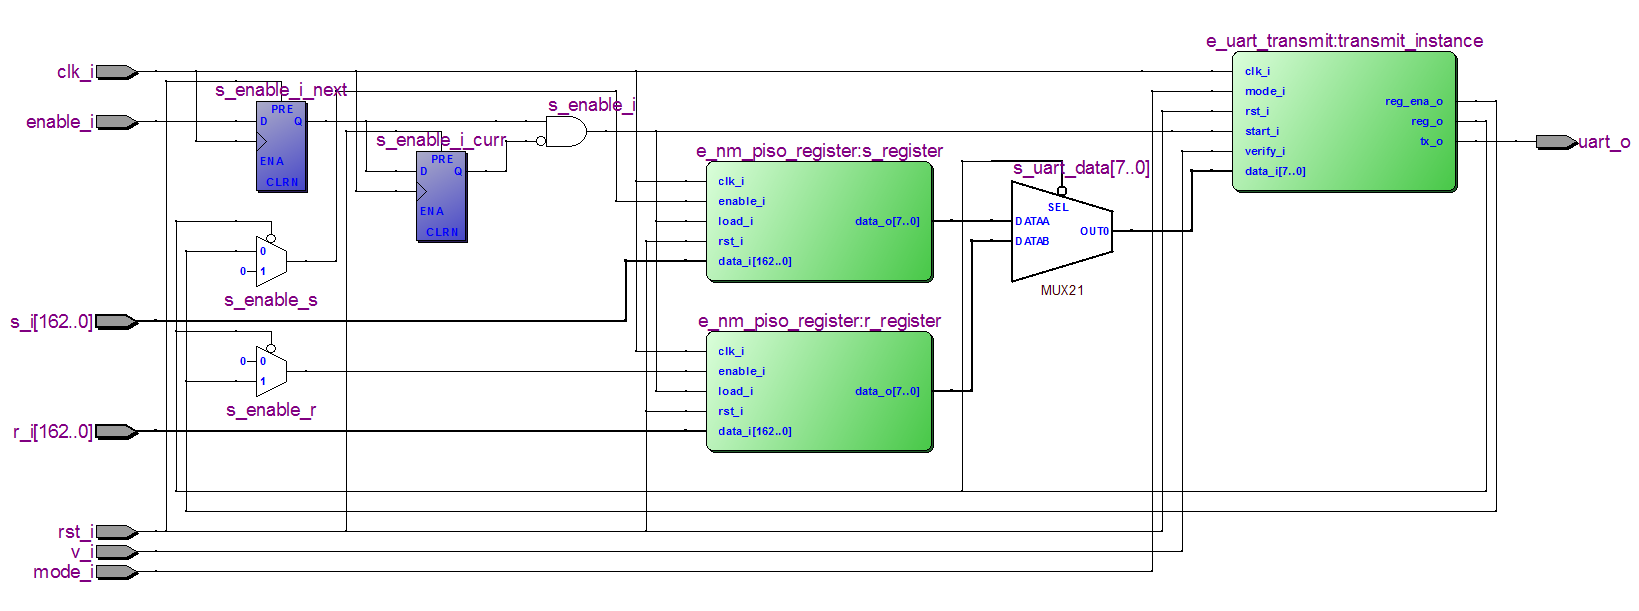
\includegraphics[width=\textwidth]{bilder/uart-transmitter}
	\caption{Ansicht des UART-Transmitter im RTL Viewer}
	\label{fig:uarttx}
\end{figure}

Im Modus Signieren sendet das Modul den in den Registern gespeicherten Punkt $(r, s)$. Beim Verifizieren wird entweder ein Byte Nullen (Signatur passt \textit{nicht} zum Dokument) oder ein Byte Einsen (Signatur gehört zum Dokument) versendet. Der Transmitter instantiiert intern einen Timer, der das Senden am Ausgang Tx in der vor der Synthetisierung eingestellten Baud-Rate taktet. \\



%%%%%%%%%%%%%%%%%%%%%%%%%%%%%%%%%%%%%%%%%%%%%%%%%%%%%%%%%%%%%
\section{Synthetisierung}

Der verwendete FPGA ist ein Baustein der Altera Cyclone II Familie (EP2C35F672C6). Für die Synthetisierung wird das in der Entwicklungsumgebung Quartus II vom selben Hersteller enthaltene Werkzeug verwendet. \\

\begin{figure}[H]
	\centering
  	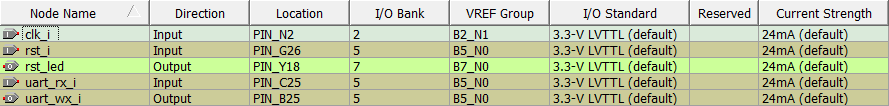
\includegraphics[width=\textwidth]{bilder/pins}
	\caption{Pin-Zuordnung des FPGA}
	\label{fig:pins}
\end{figure}

Abbildung \ref{fig:pins} zeigt die genaue Zuordnung der Pins auf dem FPGA. Für das Clock-Signal wird ein Takt von 50Mhz zugewiesen. Die für die Zielhardware synthetisierte Schaltung wird per USB auf das Board übertragen. \\


